\begin{problem}{5} ~\\
(a) If f(f(p)) = p, Algorithm B gives a factor of two approximation. If f(f(p)) is any point other than p, then the distance from f(p) to f(f(p)) must be greater than the distance from p to f(p). Therefore, Algorithm B always gives an approximation factor or two or better.\\
\\
(b) In one dimension, no matter which p is picked, f(p) will always be the point on the left or right side. Then f(f(p)) will always be the point on the other side to f(p). The distance from f(p) to f(f(p)) (from the left/right side to the right/left side) is the exact diameter for the set.\\
\\
(c)\begin{figure}[H] 
\centering 
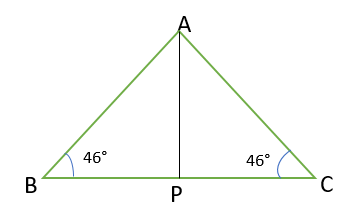
\includegraphics[width=0.6\columnwidth]{1}
\end{figure}
Illustrated by the above graph, ABC is an isosceles triangle, P is the midpoint of BC. Let p = P, then f(p) would be A, f(f(p)) would be either B or C. In fact, the diameter of the point set \{A,B,C,P\} is BC. Therefore, Algorithm B does not always produce the correct diameter in two dimensions.
\end{problem}